% !Mode:: "TeX:UTF-8"

\documentclass[12pt,oneside]{book}

\newlength{\textpt}
\setlength{\textpt}{12pt}
    
%========基本必备的宏包========%
\RequirePackage{calc,float,moresize}
%\RequirePackage[onehalfspacing]{setspace}
\linespread{1.5}
%1.3 onehalfspacing
%1.6 doublespacing

%===========加入目录 某章或某节=====%
\makeatletter

\newcommand{\addchtoc}[1]{
        \cleardoublepage
        \phantomsection
        \addcontentsline{toc}{chapter}{#1}}

\newcommand{\addsectoc}[1]{
        \phantomsection
        \addcontentsline{toc}{section}{#1}}

%===========全文基本格式==========%
\setlength{\parskip}{1.6ex plus 0.2ex minus 0.2ex}   %段落間距
\setlength{\parindent}{\textpt * \real{2}}
\RequirePackage{indentfirst} 

%=========页面设置=========%
\RequirePackage[a4paper, %a4paper size 297:210 mm
  bindingoffset=0mm,%裝訂線
  top=35mm,  %上邊距 包括頁眉
  bottom=30mm,%下邊距 包括頁腳
  inner=30mm,  %左邊距or inner
  outer=30mm,  %右邊距or  outer
  headheight=10mm,%頁眉
  headsep=15mm,%
  footskip=15mm,%
  marginparsep=0pt, %旁註與正文間距
  marginparwidth=0em,includemp=false% 旁註寬度計入width%旁註寬度
  ]{geometry}

%color
\RequirePackage[table,svgnames]{xcolor}

%================字體================%
%设置数学字体
\RequirePackage{amssymb,amsmath}
\RequirePackage{stmaryrd}
\everymath{\displaystyle}

\RequirePackage{fontspec}
%設置英文字體
\setmainfont[Mapping=tex-text]{DejaVu Serif}
\setsansfont[Mapping=tex-text]{DejaVu Sans}
\setmonofont[Mapping=tex-text]{DejaVu Sans Mono}


%中文環境
\RequirePackage[]{xeCJK}
\xeCJKsetup{PunctStyle=plain}
\setCJKmainfont[FallBack=DejaVu Serif, ItalicFont=KaiTi]{Source Han Serif CN}
\setCJKsansfont[FallBack=DejaVu Sans]{Source Han Sans CN}
\setCJKmonofont[FallBack=DejaVu Sans Mono]{KaiTi}


%%===============中文化=========%
\renewcommand\contentsname{目~录}
\renewcommand\listfigurename{插图目录}
\renewcommand\listtablename{表格目录}
\renewcommand\bibname{参~考~文~献}
\renewcommand\indexname{索~引}
\renewcommand\figurename{图}
\renewcommand\tablename{表}
\renewcommand\partname{部分}
\renewcommand\appendixname{附录}
\renewcommand{\today}{\number\year{}年\number\month{}月\number\day{}日}


%=======页眉页脚格式=========%
\RequirePackage{fancyhdr}   %頁眉頁腳
\RequirePackage{zhnumber}  %计数器中文化
\pagestyle{fancy}
\renewcommand{\sectionmark}[1]
{\markright{第\zhnumber{\arabic{section}}节~~#1}{}}

\fancypagestyle{plain}{%
    \fancyhf{}
    \renewcommand{\headrulewidth}{0pt}
    \renewcommand{\footrulewidth}{0pt}
    \fancyhf[HR]{\ttfamily \footnotesize \rightmark }
    \fancyhf[FR]{\thepage}}
\pagestyle{plain}


%=========章節標題設計=========%
\RequirePackage{titlesec}
%修改part
\titleformat{\part}{\huge\sffamily}{}{0em}{}
%修改chapter
\titleformat{\chapter}{\LARGE\sffamily}{}{0em}{}
%修改section
\titleformat{\section}{\Large\sffamily}{}{0em}{}
%修改subsection
\titleformat{\subsection}{\large\sffamily}{}{0em}{}
%修改subsubsection
\titleformat{\subsubsection}{\normalsize\sffamily}{}{0em}{}


%================目录===============%
%toc label to contents space   dynamic adjust
\RequirePackage{tocloft}%
\renewcommand{\numberline}[1]{%
  \@cftbsnum #1\@cftasnum~\@cftasnumb%
}

%==============超鏈接===============%
\RequirePackage[colorlinks=true,linkcolor=blue,citecolor=blue]{hyperref} %設置書簽和目錄鏈接等
\newcommand{\hlabel}[1]{\phantomsection \label{#1}}%某一小段的引用


%=================文字強調=========%
\RequirePackage{xeCJKfntef}

\let\oldemph\emph % Save emph in oldemph
\renewcommand{\emph}[1]{\textcolor{blue}{\textbf{#1}}}  

%==================插入圖片=======%
\RequirePackage{wrapfig}
\RequirePackage{graphicx}
\graphicspath{{figures/}}
%change the caption style a little like 1-1
\renewcommand{\thefigure}{\arabic{chapter}-\arabic{figure}}


%==============插入表格========%
\RequirePackage{booktabs}
\renewcommand{\thetable}{\arabic{chapter}-\arabic{table}}
\RequirePackage{caption}

%插入代码
\RequirePackage{fancyvrb} 
\fvset{frame=lines,tabsize=4 ,baselinestretch=1.8, fontsize=\footnotesize}


% 框线表示文章引用
\RequirePackage{mdframed} 
\mdfsetup{frametitlealignment=\center}
\newmdenv[frametitlebackgroundcolor=gray!20, linewidth=1pt,
                    frametitlerulewidth=1pt, frametitlerule=true]{bookref}
 
 
%========脚注=========%
\RequirePackage{tikz} 
\newcommand*\circled[1]{
\tikz[baseline=(char.base)]
\node[shape=circle,draw,inner sep=0.4pt,minimum size=4pt] (char) {#1};}

\newcommand*\circledarabic[1]{\circled{\arabic{#1}}}

\RequirePackage{perpage} %the perpage package
\MakePerPage{footnote} %the perpage package command

\renewcommand*{\thefootnote}{\protect\circledarabic{footnote}}

\renewcommand\@makefntext[1]{\vspace{5pt}\noindent
\makebox[20pt][c]{\fontsize{10pt}{12pt}\@thefnmark}
\fontsize{10pt}{12pt}\selectfont #1}

\setlength{\skip\footins}{20pt plus 10pt}
%main body 与脚注之间的距离

\makeatother



\title{人工智能学习书}
\author{Wander}
\hypersetup{
  pdfkeywords={},
  pdfsubject={},
  pdfcreator={Wander}}

  
\begin{document}
\maketitle


\frontmatter 
\addchtoc{前言}
\chapter*{前言}


\addchtoc{目录}
\setcounter{tocdepth}{2}    
\tableofcontents



\mainmatter



\part{绪论}

\chapter{什么是人工智能}



\appendix


\part{附录:编程知识}
编程知识介绍以markdown或者ipynb notebook的形式散落各处,而且只关注介绍28法则中那些最常用最核心的知识点,集中学习一段时间即可,后续应用中若用疑问可搜索可问AI或者查看官方文档等。


\chapter{python语言核心教程}
\href{https://a358003542.github.io/articles/python-core-tutorial.html}{python语言核心教程}



\chapter{numpy基础}
\href{https://github.com/a358003542/ipynb_notebook/blob/master/linear_algebra/numpy_basic.ipynb}{numpy basic}


\chapter{pandas基础}
\href{https://github.com/a358003542/ipynb_notebook/blob/master/linear_algebra/pandas_basic.ipynb}{pandas basic}

\chapter{matplotlib基础}
\href{https://github.com/a358003542/ipynb_notebook/blob/master/matplotlib_basic.ipynb}{matplotlib basic}

\chapter{pytorch基础}
\href{https://github.com/a358003542/ipynb_notebook/blob/master/neural_network/pytorch_basic.ipynb}{pytorch basic}




\part{附录:数学知识}
数学知识这部分内容估计后面会不断修改,这里没有什么所谓的技术应用28法则,也就是术语定义等等会尽可能详尽地阐述清楚,各个定理推导习题解答会尽可能条理清晰地写明白。


\chapter{线性代数}
\section{什么是向量}
在对事物的存在状态进行分析过程中,根据不同的分析行为得到不同的事物的属性值,这一组数据表示为 $(a, b, c...)$ ,因为人对于事物存在状态的同一性具有强烈的需求和感知,如果总是得到相同的一组数据,但是人和事物交互中却得到不同的回应,这表明这组数据并没有把目标事物的存在状态说明清楚,这组数据对于事物的描述需求来说还缺少某些维度信息。

但也存在这样的情况,有一组数据,它们有几个点上存在差异,而人和事物交互中却感受不到差异,这说明这组数据中存在冗余信息或者并没有把握住事物的核心特征。

最理想的情况是这样一组数据,这组数据要尽可能地小,并且只要有某个数据上存在差异,那么就可以说该事物的存在状态具有差异,人们就可以根据这样的差异来决定采取不同的行为;而只要这组数据逐个比对是相同的,那么就可以说该事物的存在状态是相同的,人们就可以根据该事物的存在状态的同一来采取同一的反应行为。

还存在这样的情况,两个人各自采取独立的分析行为得到了他们关于目标事物的一组数据,尽管这两组数据看起来各自区别很大,但最终人们发现这两个事物的存在状态其实是相同的,因为这两个人各自独立采取不同的分析维度,这样就确立了各自独立的分析空间下的一组数据。这给人们沟通交流带来了很大的不便。对于这样的情况就需要用到矩阵还有向量空间等等概念了,在引入这些概念之前,现在一个基本的假定就是都采取相同的分析维度行为。

在采取相同的分析维度行为的假定条件下,并假定达到了上面说的描述事物存在状态的最理想情况,我们称这组数据为\textbf{向量},这个最小的分析维度数目称之为\textbf{向量的维度}。并继而有:

\begin{itemize}
\item 所需要的维度信息已经足够了:假定存在某个必要的维度信息并没有包含进来,按照理想情况描述,最终人们也没有感受到事物的差异,这和那个维度信息是必要的假定是不符合的。
\item 并不存在某个维度信息是冗余的:假定某个维度信息是冗余的,并继而分成两种情况:一是人们观测到了该维度信息不同的情况,按照理想情况的描述,一组数据的不同就对应事物存在状态的不同,人们观测到了事物的不同,这和那个维度信息是冗余的假定是不符合的;第二个情况比较特殊,人们没有观测到该维度信息不同的情况,该维度上所有观测值都是相同的,这样该分析维度完全可以移除,这和最理想情况描述的这组数据要尽可能地小存在冲突,说明这组数据没有达到理想情况。
\end{itemize}

现在开始证明对于n维向量来说,其内的n个变量彼此是独立不相关的:

假设这n个变量中,$x_n$ 和前面的n-1个变量可能存在着某种关系,则有:

\begin{Verbatim}
f(x_1)->x_n
f(x_1, x_2)->x_n
......
\end{Verbatim}

其中任一函数映射关系成立,从中任意取一函数映射关系。现在将 $x_n$ 维度信息移除,再根据上面描述的某个函数映射关系计算而得到新的 $x_n$ 维度信息,并形成新的观测数据组,将会发现新的观测数据组和旧的观测数据组没有区别,从而得出结论 $x_n$ 维度信息是冗余的,这和上面描述的没有维度信息是冗余相冲突,所有其内n个变量彼此是独立不相关的。

\subsection{向量相等}
在相同的分析维度下:\textbf{向量相等当且仅当各个分析维度下各分量都相等}。


\section{向量加法}
请在脑海中多想象几遍下面的内容:

\begin{enumerate}
\item 射出向量 $\boldsymbol{u}$ ,从 $\boldsymbol{u}$ 的尾部射出向量  $\boldsymbol{v}$  ,绘制  $\boldsymbol{u} +\boldsymbol{v} $.
\item 从同一点射出向量 $\boldsymbol{u}$ 和向量 $\boldsymbol{v}$ ,绘制  $\boldsymbol{u} - \boldsymbol{v} $.
\item 从同一点射出向量 $\boldsymbol{u}$ 和向量 $\boldsymbol{w}$,绘制 $\boldsymbol{w} - \boldsymbol{u} $.
\item 从同一点射出向量$\boldsymbol{u}$ 和向量 $\boldsymbol{v}$,再绘制 $\boldsymbol{u} +\boldsymbol{v} $ 从而得到一个平行四边形。指出这个平行四边形上新生成的两个边一个是向量 $\boldsymbol{u}$ ,一个是向量 $\boldsymbol{v}$ ,再在这个平行四边形上绘制对角线 $\boldsymbol{u} -\boldsymbol{v} $.
\end{enumerate}

应用实践:
\begin{itemize}
\item 分析在向量空间中随便绘制两个点P0 (x0, y0,z0...) P1 (x1, y1, z1...),从P0指向P1得到一个向量,该向量的值为 (x1-x0, y1-y0, z1-z0...) .
\end{itemize}

\subsection{零向量}
任意多的向量相加,最后回到了起始点,起始点表示为向量 $\boldsymbol{u}$ ,任意多的向量相加的总和为未知向量 $\boldsymbol{a}$ ,有 $\boldsymbol{u} + \boldsymbol{a} = \boldsymbol{u}$ . 这个未知向量被称之为 零向量,也就是  $\boldsymbol{u} + \boldsymbol{0} = \boldsymbol{u}$ ,任何向量和零向量相加等于自身,后面会看到任何向量的线性组合必然包含零向量,任何向量空间也要求存在一个零向量(零元素)。

\section{向量的线性组合}

\subsection{线性组合下向量相等的判定}
如果两个向量的线性组合可以构成平面,在该线性组合上另外有两个向量,其表示成为线性组合分量的加和形式,则这两个向量相等的充分必要条件是这两个向量在对应线性组合分量上都依次相等。

证明如下:

有向量$P_0 = c\boldsymbol{u} + d\boldsymbol{v}$,有向量 $P_1 = k\boldsymbol{u} + w\boldsymbol{v}$ 。并且有 $u = (x1, x2...)$ , $v = (y1, y2...)$ 。

于是
$P_0 = (cx_1+dy_1, cx_2+dy_2...)$

$P_1 = (kx_1+wy_1, kx_2+wy_2...)$

按照向量相等的定义,则有:


\begin{align*}
cx_1+dy_1 = kx_1 + wy_1\\
cx_2+dy_2 = kx_2 + wy_2
......
\end{align*}

继续证明:
\begin{figure}[H]
\centering
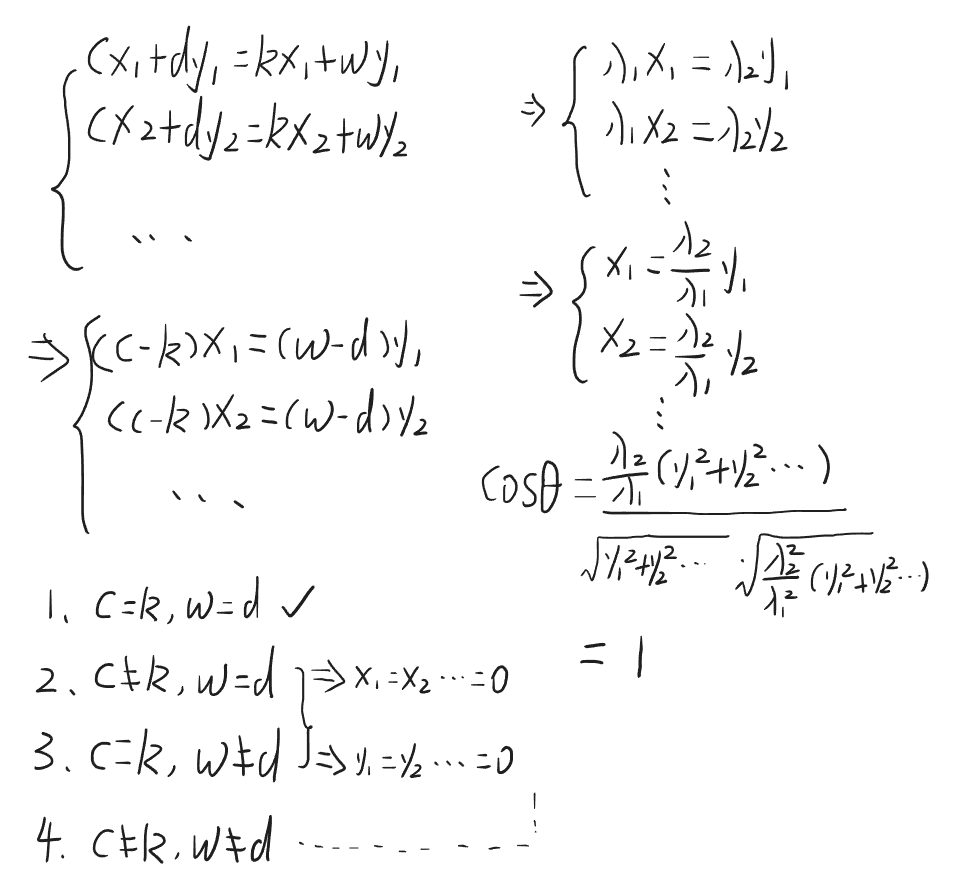
\includegraphics[width=\linewidth ,totalheight=0.95\textheight , keepaspectratio]{线性组合下向量相等的判定.png}
\caption{线性组合下向量相等的判定}
\end{figure}

上面1234四种情况,第一种情况正是我们要证明的,而第二种和第三种情况可以推出某个向量为零向量,这和条件该线性组合可以形成平面冲突。第四种情况可以证明这两个向量的夹角是零,也就是这两个向量是平行的,这也和条件冲突,于是得证。


\subsection{问题集1.1第6题}
\cite{线性代数引论}问题集1.1第6题,作者内心一个潜藏的推理思路是:如果向量的线性组合,可以从中发现某些普遍规律,也就是找到某种关系,使得这个关系不依赖参数c、d...等,那么这个普遍规律对于该线性组合下的所有点都是成立了。【我们太习惯某个事物的局部或者某些特殊情况会更简单一些,常常会忘了在某些时候(这种情况确实很罕见,但也是存在的),该事物从全局从一般情况思考会更简单一些,发现一些普适性的规律,然后自然那些局部的点特殊的情况也一应得到证明了。】

\subsection{问题集1.1第15题}
\cite{线性代数引论}问题集1.1第15题的 $\frac{3}{4}\boldsymbol{v} + \frac{1}{4}\boldsymbol{w}$ 为什么一定在对角线上,证明如下:

\begin{figure}[H]
\centering
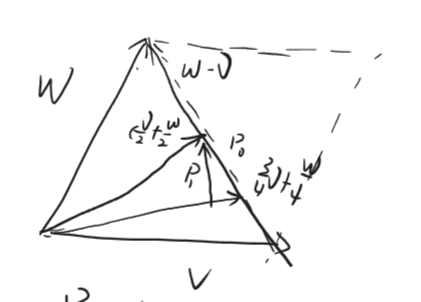
\includegraphics[width=\linewidth ,totalheight=0.95\textheight , keepaspectratio]{线性代数引论问题集1_1_15.png}
\caption{线性代数引论问题集1.1.15}
\end{figure}

已知该对角线为 $\boldsymbol{w} - \boldsymbol{v}$,标记该向量为 $P_0$,现在假定$\frac{3}{4}\boldsymbol{v} + \frac{1}{4}\boldsymbol{w}$ 射出去之后并没有落在对角线上,从而根据$\frac{1}{2}\boldsymbol{v} + \frac{1}{2}\boldsymbol{w}$ 和$\frac{3}{4}\boldsymbol{v} + \frac{1}{4}\boldsymbol{w}$ 的终点确立向量 $P_1$。【已经证明了$\frac{1}{2}\boldsymbol{v} + \frac{1}{2}\boldsymbol{w}$的终点是落在那条对角线的中点的,这很简单,用简单的三角几何分析即可。】

\begin{align*}
P_1 &= \frac{v}{2} + \frac{w}{2} - (\frac{3v}{4} + \frac{w}{4}) \\
    &= -\frac{1}{4}v + \frac{w}{4} \\
    &= \frac{1}{4}(w-v) \\    
 => P_1 // P_0
\end{align*}

因为 $\frac{1}{2}\boldsymbol{v} + \frac{1}{2}\boldsymbol{w}$ 在那条对角线的上,所以 $\frac{3}{4}\boldsymbol{v} + \frac{1}{4}\boldsymbol{w}$ 一定在这条对角线上。上面的证明过程还证明了 $P_1$ 的长度是1/4对角线长度,其终点位置刚好是对角线下面1/4的位置。

上面的证明还可以继续推广,问向量$\boldsymbol{v}$和向量$\boldsymbol{w}$组成的线性组合$c\boldsymbol{v} + d\boldsymbol{w}$ ,$c$和$d$满足何种约束条件就能让其都落在中间那条对角线也就是 $\boldsymbol{w} - \boldsymbol{v}$ 上。

证明如下,其中用到了上面提及的线性组合下向量相等的判定:

\begin{figure}[H]
\centering
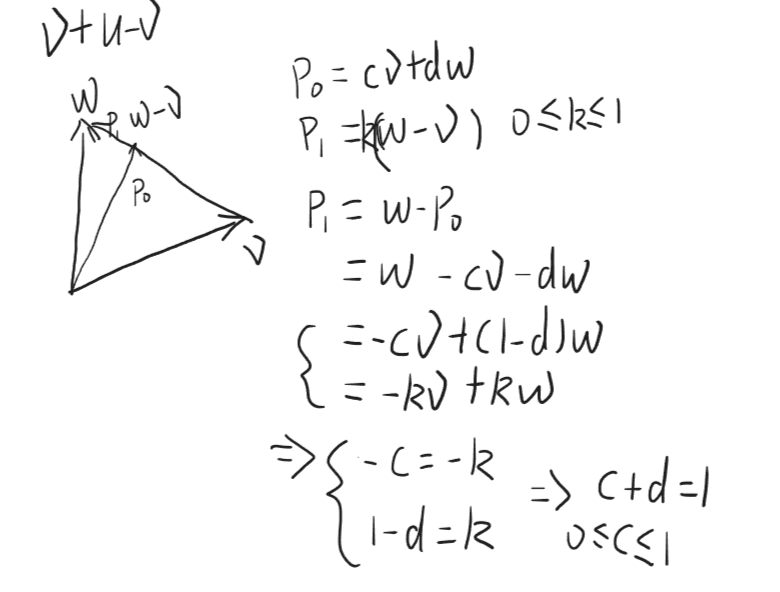
\includegraphics[width=\linewidth ,totalheight=0.95\textheight , keepaspectratio]{线性代数引论问题集1_1_15_2.png}
\end{figure}

最终得证:向量 $P_0 = c\boldsymbol{v}+d\boldsymbol{w}$ ,该向量如果满足 $c+d=1$的条件,则射出去的向量落点会落在中间那条对角线上。


\cite{线性代数引论}问题集1.1第20题将上面讨论的情况扩展到了三个向量的线性组合,问这三个向量的线性组合中,某个向量的系数满足何种条件,该向量的落点在这三个向量终点构成的三角形平面上,有了前面的基础,就很容易得证了。


\begin{figure}[H]
\centering
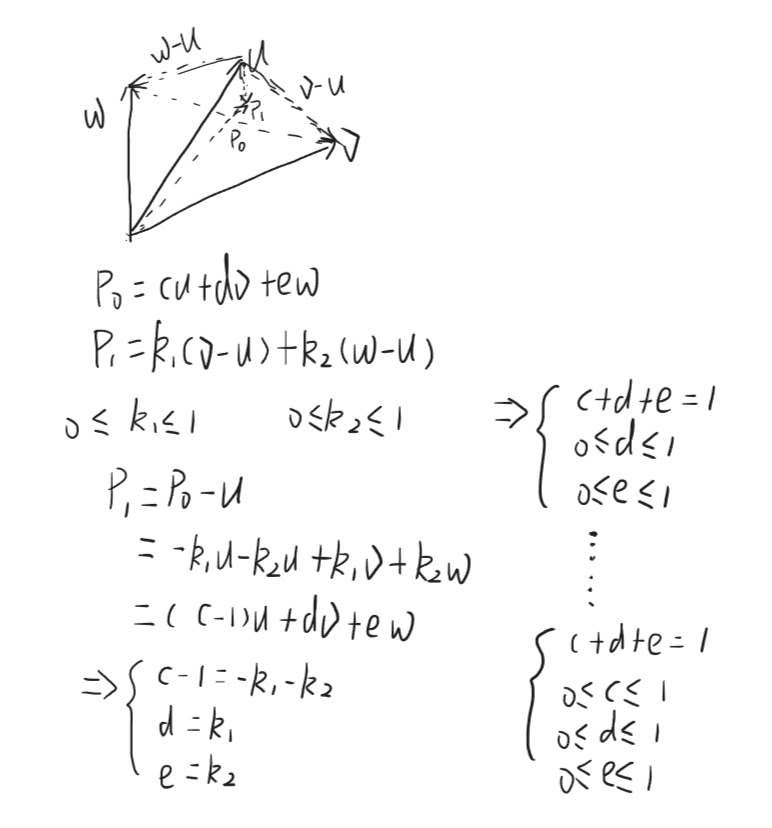
\includegraphics[width=\linewidth ,totalheight=0.95\textheight , keepaspectratio]{线性代数引论问题集1_1_20.png}
\end{figure}


\chapter{术语}
\subsection{当且仅当}
A当且仅当B:如果A成立则B成立 ,并且如果A不成立则B不成立【等价于如果B成立则A成立】。

如果命题只有真或者假两种可能性,在所有情况下真值都相同,所以A不成立则B不成立等价于如果B成立则A成立。

\begin{table}[H]
\begin{tabular}{@{}llllll@{}}
\toprule
{A} & {B} & {¬A} & {¬B} & {¬A→¬B} & {B→A} \\ \midrule

{T}          & {T} & {F}  & {F}  & {T}     & {T}   \\
\rowcolor[HTML]{FFFFFF} 
{T}          & {F} & {F}  & {T}  & {T}     & {T}   \\
\rowcolor[HTML]{FFFFFF} 
{F}          & {T} & {T}  & {F}  & {F}     & {F}   \\
\rowcolor[HTML]{FFFFFF} 
{F}          & {F} & {T}  & {T}  & {T}     & {T}   \\ \bottomrule
\end{tabular}
\end{table}





\backmatter
\chapter*{参考资料}
\addchtoc{参考资料}
\begin{thebibliography}{99}
\bibitem[线性代数引论]{线性代数引论} 《Introduction to Linear Algebra 5e》 by Gilbert Strang at 2016 .
\bibitem[Dive into Deep Learning](Dive into Deep Learning) 《Dive into Deep Learning》 by Aston Zhang \& Zachary C. Lipton \& Mu Li \& Alexander J. Smola at 2023.

\end{thebibliography}
\end{document}


